\documentclass{article}
\usepackage[utf8]{inputenc}
\usepackage[T1]{fontenc}
\usepackage{titlesec}

\titleformat*{\subsection}{\large}

% SET THESE PARAMETERS
\newcommand{\course}{EE364B, Spring 2023}
\newcommand{\problem}{Final Report}

\usepackage{geometry}
\geometry{left=20mm,top=20mm,}

\usepackage{fancyhdr}
\usepackage{comment}
\usepackage{amsfonts}
\usepackage{amsmath}
\usepackage{amsthm}
\usepackage{graphicx}
\usepackage{caption}
\usepackage{subcaption}
\usepackage{tikz}
\usepackage{hyperref}
\usepackage{url}
\usepackage{booktabs}
\usepackage{datetime}
\usepackage{minted}
\pagestyle{fancy}
\usepackage{algorithm}
\usepackage{algpseudocode}

\usepackage[
backend=biber,
style=alphabetic,
sorting=ynt
]{biblatex}

\renewcommand{\thesubsection}{\thesection.\alph{subsection}}

\newdateformat{monthyeardate}{%
  \monthname[\THEMONTH] \THEYEAR}

\input tex/defs.tex
\addbibresource{tex/references.bib}

\newcommand\numberthis{\addtocounter{equation}{1}\tag{\theequation}}

\setlength{\parindent}{0pt}

\title{{\large \bf Decentralized Optimization Task Assignment for Robot Package Delivery}}
\author{Name: Oscar Eriksson \\ SUNet ID: oscer \\ \texttt{oscer@stanford.edu}}
\date{\monthyeardate\today}

\newcommand{\sectiontype}{}

\fancyhead{}\fancyfoot{}
\fancyhead[L]{\sectiontype \text{ --} \course}
\fancyhead[R]{Oscar Eriksson, \texttt{oscer@stanford.edu}}
\newcommand{\sectionUpdate}[1]{\renewcommand{\sectiontype}{#1} \fancyhead[L]{\sectiontype \text{ --} \course}}

\begin{document}

\maketitle
\section*{Introduction}
\renewcommand{\sectiontype}{Introduction}
The field of distributed optimization is ripe, and a great deal of time is spent developing distributed optimization algorithms that can make improvements of convergence rates over other methods, given that one finds structure in the problem. There is however not very many examples of applications within robotics, with \cite{haksar2022consensus}, \cite{shorinwa2020distributed} and \cite{jadbabaie2003coordination} being some examples. This paper aims to apply distributed methods on a problem in robotics directly, and letting it play out in real time in a simulated environment. We present a problem setting in which bots are to pick up and deliver packages subject to charge constraints. They operate using very simple dynamics and trajectory planning with no collision avoidance. A shared objective function to be minimized is presented where each bots task assignment make up the optimization variables. A relaxation of the shared objective is proposed, for which various decentralized methods are derived including co-estimation of the fastest mixing matrix on a graph.

\subsubsection*{Related Work}
One example of distributed task assignment is found in \cite{shorinwa2023distributed} in which a version consensus ADMM which does not require a central synchronized host is used to solve a task assignment problem with a linear objective such as \eqref{eq:objective_function}. It reviews the use of the planning in a simulated system as well, and runs the algorithm every few iterations.
The subject of the fastest mixing matrix on a graph is discussed in \cite{xiao2004fast}, and faster averaging methods are presented in \cite{johansson2008faster} yet not implemented. There is discussion regarding the convergence rate of decentralized algorithms subject to slowly varying graphs, as well as time varying functions in \cite{rogozin2019optimal} where they state the assumptions under which these algorithms converge, though it is not possible to transpose the analysis to this setting.

\subsubsection*{Contribution}
In this paper fixed point iterations are derived that may run in real time, allowing the relaxed objective and the graph structure to change during the course of the algorithm, while maintaining stability and performance. In this sense the planning is applied like the controls of a dynamical system, rather than a regularly scheduled subroutine.

To address the fact that communication is the bottleneck of this system we propose the co-estimation of the fastest mixing matrix along with the objective value to make better use of the transmitted data and show it's improvements on the baseline approach.

\section*{Problem Setup}
\renewcommand{\sectiontype}{Problem Setup}
The particular problem instance that we are considering is one with $B$ bots at positions $x \in \RR^{B\times2}$ with charge $U \in [0,1]^{B}$, that are to deliver $M$ packages from pick-up points $P \in \RR^{M\times2}$ to drop-off points $Q \in \RR^{M\times2}$. The time that a mission $m$ has been available is denoted $T_m$, and resets (to zero) when a mission is completed. Bots move in a straight line towards their objectives and a displacement $\Delta$ results in a charge draw of $\Delta \eta$. If a bot is running low on charge it should go to a charging location $C \in \RR^{C\times2}$ and charge at some constant rate. Each bot $b$ moves according to a local task assignment matrix $\tau_b \in \{ 0, 1 \}^{B \times (M+C)}$ with $\tau_{bt}$ being 1 if the bot has been tasked to got to the mission or charger $t$. $\tau$ is furthermore constrained such that at most one task is assigned to at most one bot. 
\newline

\text{\bf Knowledge of mission status.} If a package is picked up then the mission is no longer available for other bots. If a charger is occupied it will not be available until the bot is fully charged. The status of chargers and missions are described by $K\in \{ 0, 1 \}^{M+C}$. $(P, Q, C, K, T)$ are instantaneously transmitted to each active agent regardless of their position, and any time a delivery is completed another pick-up emerges at some random location so that there always are $M$ missions available. \newline

\text{\bf Communication between bots.} Communication between bots is constrained to channels represented by a finite connected graph with no self-loops $G$ with vertices $i \in V$ corresponding to each bot, and edges $\{i,j\} \in E$. It may be represented by an adjacency matrix $A\in\{0,1\}^{B \times B}$ such that $A_{ij} = 1$ if $\{i,j\}\in E$ and $A_{ij} = 0$ if $\{i,j\}\not\in E$. Bots are connected with the $I$ closest bots at any point in time. Communication occurs every $\Delta T$ seconds. \newline

\text{\bf Shared objective function. } The shared objective among the bots is to deliver as many packages as possible without neglecting difficult missions. The shared objective is thus
\begin{align*}
    \underset{\tau_1,...,\tau_b \in \{0,1\}^{B\times(M+C)}}{\text{minimize }}
        \int_0^\infty \sum^{M}_{m=1} T_m dt
        \numberthis \label{eq:shared}
\end{align*}

\section*{Centralized Relaxation}
\renewcommand{\sectiontype}{Centralized Relaxation}
We allow each bot to produce an objective vector $L^{b} \in \RR^{M+C}$ which encodes the bots wish to go to a certain mission or charger at the instance that the vector is produced. The composition of all $L^{b}$ is denoted $L\in\RR^{B\times(M+C)}$. We define this as $L = \begin{bmatrix}\ \vM\  \vC\  \end{bmatrix} \in \RR^{B \times M + B \times C}$ as
\begin{align*}
    \vM_{bm}
    =
    \begin{cases}
        -1/(1+D_{bm}) - \mu T_m & \text{ if } U_b > \eta D_{bm} + 0.2 \\
        1 & \text{ else }
    \end{cases},\quad
    \vC_{bc}
    =
    \begin{cases}
        -1/(1+D_{bc}) & \text{ if } 0.8 \geq U_b \geq \eta D_{bc},\ \vM_b = \vone \\
        1 & \text{ else }
    \end{cases}
\end{align*}
where $D_{bm}$ is the shortest possible distance bot $b$ has to traverse in order to pick up, drop off and reach a charging station, and $D_{bc}$ is the distance from bot $b$ to charger $c$. $\mu T_m$ is the time that a mission has been available scaled by a parameter $\mu$, which penalizes bots ignoring difficult missions. We also define $\vL \in \RR^{B\times B \times (M+C)}$ such that $\vL_{bbm} = L^{b}_m$ (all other elements zero), where $\vL_b$ corresponds to the exact knowledge of bot $b$. \newline

\text{\bf Interpretation. } Elements in $\vM$ are negative if the bot has enough charge to complete that mission and get to a charger afterwards, and the reward is greater for completing mission that are nearby yet have been active for long. Elements in $\vC$ are negative when no missions are available and the charge low enough to warrant charging yet enough to make it to the charger. \newline

\text{\bf Centralized problem. } 
If we ignore the constraint on communication between bots, and allow for complete information we may elect to solve the following centralized relaxation problem
\begin{align*}
    \underset{\tilde{\tau}_b \in \RR^{B \times (M+C)}}{\text{minimize }} &  \langle \tilde{\tau}_b, L \rangle + \delta_T(\tilde{\tau}_b),\quad
    T = \{\ \tau \in \RR^{B \times (M+C)} \mid 0 \preceq \tau,\ \tau\vone \preceq 1,\ \tau^\T\vone \preceq 1\ \}
    \numberthis \label{eq:objective_function}
\end{align*}
using $\langle A, B \rangle = \sum_{i,j} A_{ij}B_{ij}$, and defining $T\subseteq\RR^{B\times(C+M)}$, the subspace of inexact task assignment matrices where each bot has at most one task and each task has at most one bot. We use the indicator function $\delta_A(x)$ which is equal to plus infinity if $x \not\in A$ and zero otherwise. It is easy to see that $\text{\bf conv } \{0,1\}^{B\times(M+C)} = T$, and given that entries of $L$ are not equal we will find the optimal solution to \eqref{eq:objective_function} to be a vertex of $T$ (an exact binary assignment).

\section*{Decentralized Relaxation}
\renewcommand{\sectiontype}{Decentralized Relaxation}
We now introduce stacking notation \cite{ryu2022large}, such that 
\begin{align*}
    \vtau = \begin{bmatrix}
        \tau_1 \\ \tau_2 \\ \vdots \\ \tau_B
    \end{bmatrix},\quad
    \prox_{\partial f}(\vtau)
    =
    \begin{bmatrix}
        \prox_{\partial f_1}(\tau_1) \\ \prox_{\partial f_2}(\tau_2) \\ \vdots \\ \prox_{\partial f_B}(\tau_B)
    \end{bmatrix}
\end{align*}
which allows us to express the decentralized task assignment problem as 
\begin{align*}
    \underset{\tilde{\vtau} \in \RR^{B \times B \times (M+C)}}{\text{minimize }} & \sum^B_{b=1}\langle \tilde{\vtau}_b, \vL_b \rangle + \delta_T(\tilde{\vtau}) + \delta_O(\tilde{\vtau}),\quad
    O = \{\ \tau \in \RR^{B\times (M+C)} \mid \tau = \tau_1 = \tau_2 = ... = \tau_B\ \}
    \numberthis \label{eq:objective_function_alt}
\end{align*}
where $O$ is the consensus set defined such that all matrices contained are equal in values. In this case each bot only has access to it's own objective vector. \newline

\text{\bf Consensus through mixing matrices. } Consensus constraints may be implemented using mixing matrices $W\in\RR^{B\times B}$.
Any mixing matrix \cite{xiao2004fast} should satisfy
\begin{align*}
    \cN(I - W) = \text{span} (\vone),\ \sigma_\text{max}(W) = 1,\ (\vone\vone^\T - A) \odot W = 0
\end{align*}
where the first criterion makes sure that averaging algorithms reach consensus ($\vx_i^\star = \vx_j^\star\  \forall i,j$ and $\vx^{k+1} = W\vx^k$ if and only if $(I-W)\vx^\star = 0$). The second criterion makes sure that averaging operations are non expansive and the third criterion makes sure that the mixing matrix is a decentralized mixing matrix corresponding to the adjacency matrix $A$ ($\odot$ denotes element wise multiplication). We define the space of all these decentralized mixing matrices $\cW(A) \subseteq \RR^{B \times B}$. We claim that the rate of convergence of data averaging is roughly $\approx\sigma_{\text{max}}(W-U)$, the greatest singular value (being used as an approximation of the spectral radius) of the difference of the mixing matrix and the uniform matrix $U = \vone\vone^\T/B$. If not specified a mixing matrix which only uses known local information may be assumed to be
\begin{align*}
    W_{ij} = \begin{cases}
        A_{ij} / \sum_j A_{ij} \text{ if } \sum_j A_{ij} > 0 \\
        0 \text{ else }
    \end{cases}\numberthis\label{eq:unicoorooron}
\end{align*}


\text{\bf Decentralized consensus problem. } We may approximate $\delta_O(\vtau)$ with $\frac{1}{2\alpha}\|\vtau\|^2_{I-W}$ ($\alpha > 0$), since these expressions both evaluate to zero under consensus. We thus find the problem
\begin{align*}
    \underset{\tilde{\vtau} \in \RR^{B \times B \times (M+C)}}{\text{minimize }} & \sum^B_{b=1}\langle \tilde{\vtau}_b, \vL_b \rangle + \delta_T(\tilde{\vtau}_b) + \frac{1}{2\alpha}\|\tilde{\vtau}_b\|^2_{I-W}
    \numberthis \label{eq:objective_function_pgd}
\end{align*}
A fixed point iteration can be found by setting the subdifferential of the above objective function to zero
\begin{align*}
    0 \in \alpha \vL + \alpha \opN_T(\tilde{\vtau}) + (I-W)\tilde{\vtau}
    \iff
    \tilde{\vtau} \in (I + \alpha \opN_T)^{-1}(W\vtau - \alpha \vL)
    \iff
    \tilde{\vtau}^{k+1} = \Pi_T(W\tilde{\vtau}^{k} - \alpha \vL)
    \numberthis \label{eq:fpi1}
\end{align*}
which gives us our first fixed point iteration. The optimal value of this fixed point iteration is not a vertex of $T$, and as such we find our task assignments in $\vtau$ below
\begin{align*}
    \vtau_{rbp} = \begin{cases}
        1 & \text{ if } p = \argmax \tilde{\vtau}_{rb} \\
        0 & \text{ else }
    \end{cases}.
\end{align*}

\text{\bf Faster mixing matrices. } We recognize that we may theoretically be able to increase the speed at which the averaging converges by finding a mixing matrix $W$ which minimizes the spectral radius $\rho(W-U)$ \cite{olshevsky2009convergence}. We pose the following problem
\begin{align*}
    \underset{\tilde{\vW} \in \RR^{B \times B \times B}}{\text{minimize }} & \sum^B_{b=1} \rho(\tilde{\vW}_b - U) + \delta_{\cW(A^b)}(\tilde{\vW}_b) + \frac{1}{2\alpha}\|\tilde{\vW}_b\|^2_{I-\tilde{\vW}_b}
    \numberthis \label{eq:mixing_problem_distt}
\end{align*}
This is clearly not convex, and as such we pose the following sequential convex optimization problem
\begin{align*}
    \tilde{\vW}_b^{k+1} = \underset{\vW \in \RR^{B \times B \times B}}{\text{argmin }} & \sum^B_{b=1} \rho(\vW_b - U) + 
    \delta_{\cW(A^b)}(\vW_b)+ \frac{1}{2\alpha}\|\vW_b\|^2_{I-\tilde{\vW}^k_b}
    \numberthis \label{eq:mixing_problem_seq}
\end{align*}
The spectral radius $\rho(\cdot)$ will have approximately the same zeros as $\lambda^2_\text{max}(\cdot)$ \cite{xiao2004fast}. We find this functions derivative in
\begin{align*}
    \lambda^2_\text{max}(X) &= \underset{v:v^Tv=1}{\text{max }} (v^TXv)^2 \\
    \nabla \lambda^2_\text{max}(X)
    &=
    \lambda_\text{max}(X) qq^T,\ q = \underset{v:v^Tv=1}{\text{argmax }} (v^TXv)^2 
\end{align*}
which may have poor numerical performance around $\lambda^2_\text{max}(X) = 0$. We use Runge-Kutta methods \cite{butcher2007runge} to define the function $\nabla \lambda^2_\text{RK4}(\alpha, X)$ below
\begin{align*}
    k_1 = \lambda^2_\text{max}(X),\ 
    k_2 = \lambda^2_\text{max}(X + \frac{\alpha}{2} k_1),\ &
    k_3 = \lambda^2_\text{max}(X + \frac{\alpha}{2} k_2),\ 
    k_4 = \lambda^2_\text{max}(X + \alpha k_3),\\
    \nabla \lambda^2_\text{RK4}(\alpha, X) &= \frac{\alpha}{6}(k_1 + 2k_2 + 2k_3 + k_4) \numberthis \label{eq:eigstep}
\end{align*}
which we will use instead of $\nabla \rho(X)$. We find the optimality condition of \eqref{eq:mixing_problem_seq} in
\begin{align*}
    0 \in \alpha \nabla \rho(\vW_b - U) + 
    \alpha \opN_{\cW(A^b)}(\vW_b)+ (I - \tilde{\vW}^k_b)\vW_b
\end{align*}
from which we may find a fixed point iteration
\begin{align*}
    0 \in \alpha \partial \rho(\vW_b - U) + 
    \alpha \opN_{\cW(A^b)}(\vW_b) &+ (I - \tilde{\vW}^k_b)\vW_b
    \\
    &\iff
    \vW_b \in \opJ_{\cW(A^b)}(\tilde{\vW}^k_b \vW_b - \nabla \lambda^2_\text{RK4}(\alpha, \vW_b - U)) \\
    &\iff
    \tilde{\vW}^{k+1}_b = \Pi_{\cW(A^b)}(\tilde{\vW}^k_b \tilde{\vW}^k_b - \nabla \lambda^2_\text{RK4}(\alpha, \tilde{\vW}^k_b - U))
    \numberthis \label{eq:fpiW}
\end{align*}
Composing \ref{eq:fpiW} and \ref{eq:fpi1} we may get the following sequential convex optimization algorithm
\begin{align*}
    \begin{cases}
        \tilde{\vtau}_b^{k+1} = \Pi_T(\tilde{\vW}_b^k\tilde{\vtau}_b^{k} - \alpha \vL_b)\\
        \tilde{\vW}_b^{k+1} = \Pi_{\cW(A^b)}(\tilde{\vW}_b^k \tilde{\vW}_b^k - \nabla \lambda^2_\text{RK4}(\alpha, \tilde{\vW}^k_b - U))
    \end{cases}
    \numberthis \label{eq:pgd_no_share}
\end{align*}


\text{\bf Sharing objective vectors. } Mixing matrices are especially appropriate for data averaging, and as such we propose sharing the gradient $\vL$. We pose the following optimization problem
\begin{align*}
    \underset{\tilde{\vL} \in \RR^{B \times B \times (M+C)}}{\text{minimize }} \delta_{\cL}(\tilde{\vL}) + \frac{1}{2 \alpha}\|\tilde{\vL}\|_{I-W},\ 
    \cL = \{ \vL \in \RR^{B \times B \times (C+M)}\mid \vL_{bb} = L^{b} \}
    \numberthis \label{eq:objective_function_alt}
\end{align*}
$\cL$ makes it so that bot $b$ enforces it's knowledge of $L^b$ (the objective vector it just produced).
We state the optimality condition and find the following fixed point iteration
\begin{align*}
    0 \in \alpha \opN_{\cL}(\tilde{\vL}) + (I - W)\tilde{\vL}
    &\iff
    W\tilde{\vL} \in (I + \alpha \opN_{\cL})\tilde{\vL}
    \iff
    \tilde{\vL} \in \opJ_{\cL}(W\tilde{\vL}) 
\end{align*}
where $\opN$ denotes the normal cone operator and $\opJ$ denotes the resolvent \cite{ryu2022large}. Using this $\tilde{\vL}$ we may calculate the optimal $\tilde{\vtau}$ every time step. We write the following fixed point iteration
\begin{align*}
    \begin{cases}
    \tilde{\vtau}_b^{k+1} = \underset{\tau \in \RR^{B\times B\times(C+M)} }{\text{argmin }} \langle \tau, \tilde{\vL}_b^k \rangle + \delta_T(\tau) \\
    \tilde{\vL}^{k+1} = \Pi_{\cL}(W\tilde{\vL}^{k})
    \end{cases}
    \numberthis \label{eq:fpi3}
\end{align*}

\text{\bf Sharing adjacency vectors. }
We estimate a $\vW$ and a $\vA$ analogously to $\vtau$ and $\vL$ above in the following optimization problem
\begin{align*}
    \underset{\tilde{\vA},\tilde{\vW} \in \RR^{B \times B \times B}}{\text{argmin }} 
    \sum^B_{b=1} \rho(\tilde{\vW}_b-U) + \frac{1}{2\alpha}\|\tilde{\vA}_b\|_{I-\tilde{\vW}_b} + \delta_{\cA}(\tilde{\vA}) +
    \delta_{\cW(\vA_b)}(\tilde{\vW}_b), 
    \cA = \{ \vA \in \RR^{B \times B \times B}\mid \vA_{bb} = A^{b} \}
    \numberthis \label{eq:objective_function_mix}
\end{align*}
which is not convex. $\cA$ makes it so that bot $b$ enforces it's knowledge of $A^b$ (what other bots it has communication with). We instead elect to solve the sequential convex optimization problem
\begin{align*}
    (\tilde{\vA}^{k+1}, \tilde{\vW}^{k+1}) = 
    \underset{\vA, \vW \in \RR^{B \times B \times B}}{\text{minimize }} & 
    \sum^B_{b=1} \rho(\tilde{\vW}_b-U) + \frac{1}{2\alpha}\|\vA_b\|_{I-\tilde{\vW}^k_b} + \delta_{\cA}(\vA) +
    \delta_{\cW(\tilde{\vA}^k_b)}(\vW_b)
    \numberthis \label{eq:objective_function_mix_scp}
\end{align*}
with optimality conditions
\begin{align*}
    0 \in \partial \rho(\tilde{\vW}_b-U)
     + \opN_{\cW(\tilde{\vA}^k_b)}(\vW_b)
    ,\ 
    0 \in (I-\tilde{\vW}_b^k)\vA + \alpha \opN_{\cA}(\vA_b).
\end{align*}
 Since these optimality conditions have separated $\vW$ from $\vA$ we optimize with respect to each condition independently. Following the derivation of \eqref{eq:fpi3} we may arrive at
\begin{align*}
    \begin{cases}
    \tilde{\vtau}_b^{k+1} = \underset{\tau \in \RR^{B\times(C+M)} }{\text{argmin }} \langle \tau, \tilde{\vL}_b^k \rangle + \delta_T(\tau) \\
    \tilde{\vL}_b^{k+1} = \Pi_{\cL}(\tilde{\vW}_b^{k}\tilde{\vL}_b^{k})\\
    \tilde{\vW_b}^{k+1} = \underset{W \in \RR^{B\times B\times B} }{\text{argmin }} \rho(W-U) + \delta_{\cW(\tilde{\vA}^k_b)}(W) \\
    \tilde{\vA}_b^{k+1} = \Pi_{\cA}(\tilde{\vW}_b^{k}\tilde{\vA}_b^{k})
    \end{cases}.
    \numberthis \label{eq:fpi4}
\end{align*}

\section*{Results}
\renewcommand{\sectiontype}{Results}
The objective heuristic performs well as one can tell that bots seldom run out of charge in figure \ref{fig:charges}.
\begin{figure}[h]
    \centering
  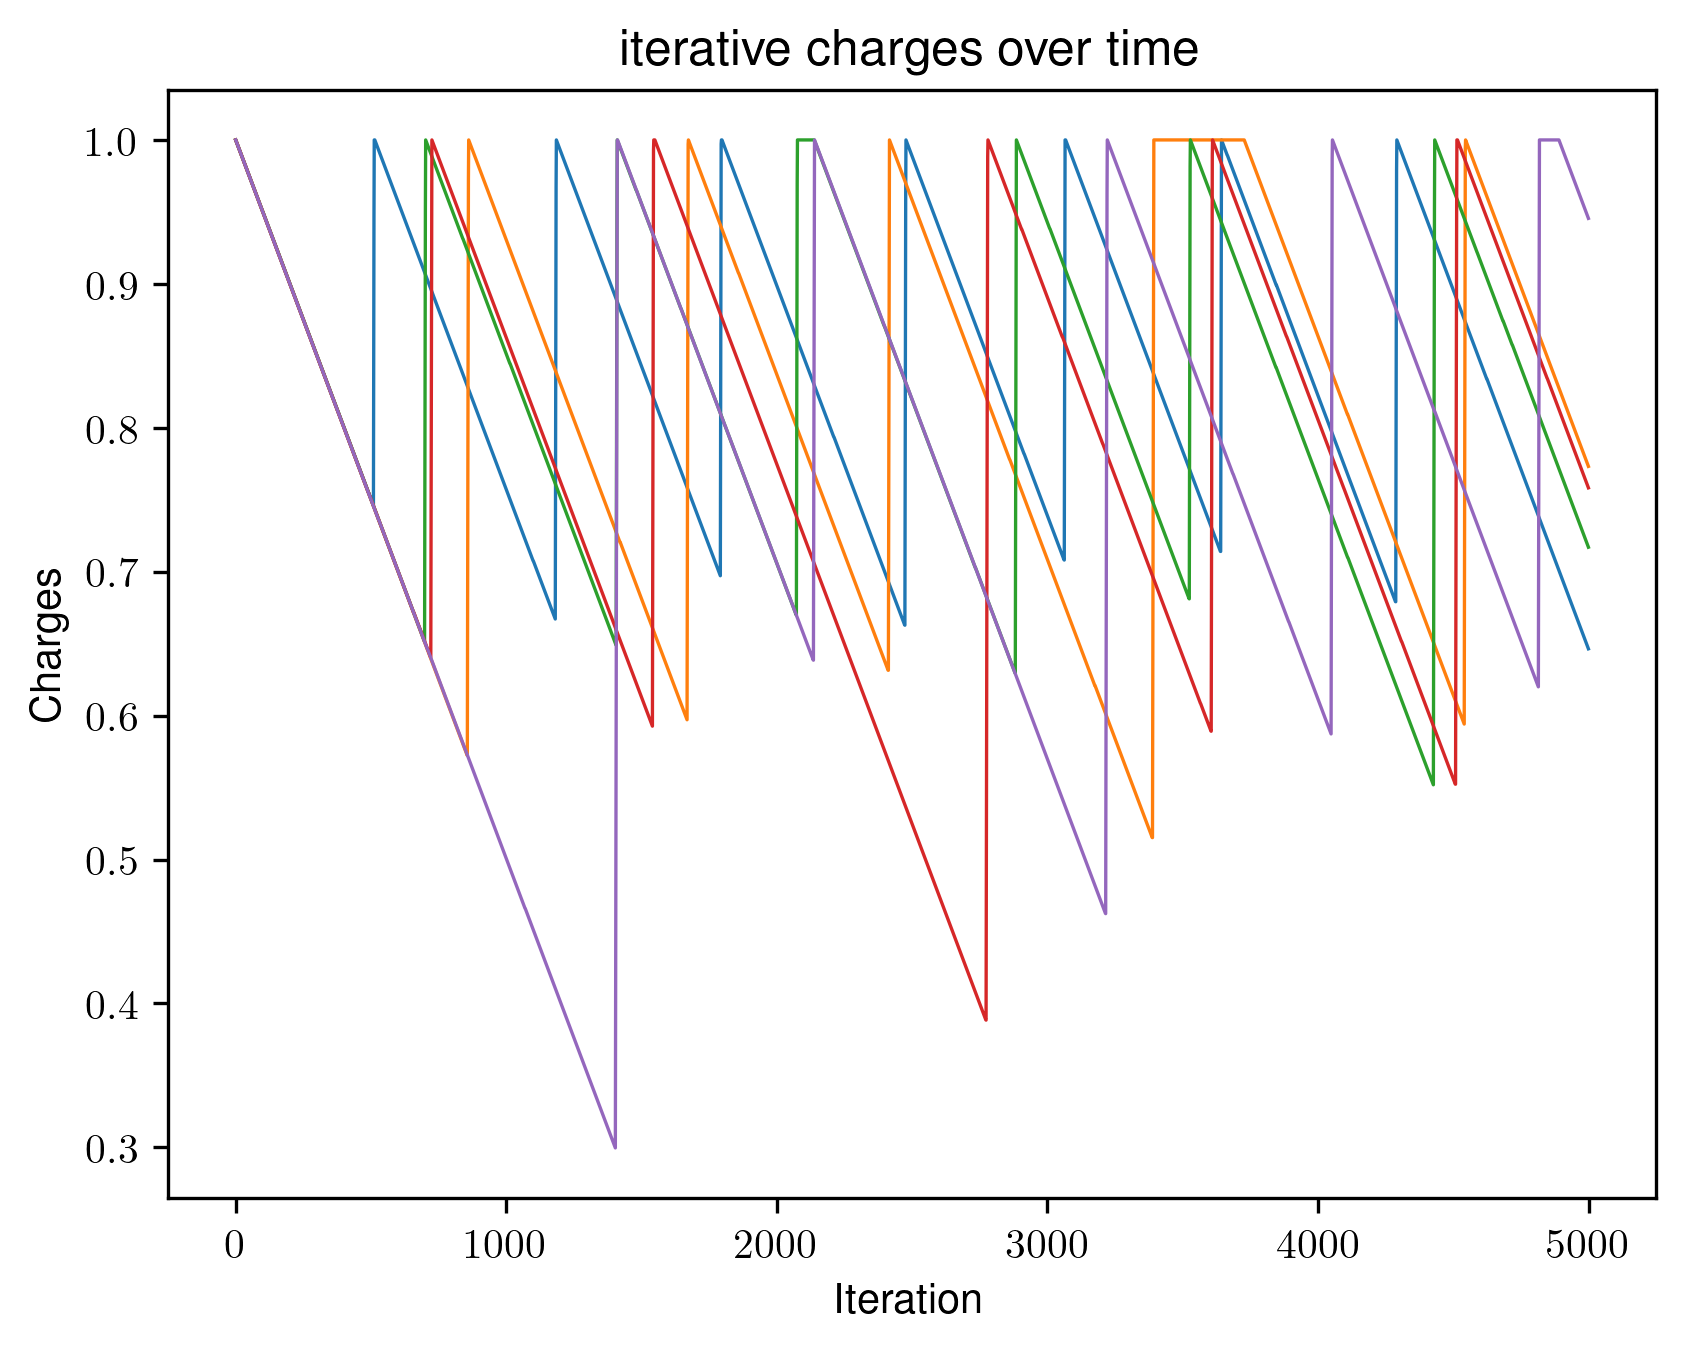
\includegraphics[width=0.35\linewidth]{tex/charges.png}
    \caption{Charge of the bots every iteration for $B = 5$, $M = 5$, $C = 3$, $I=3$, $\Delta T = 0.05$. }
  \label{fig:charges}
\end{figure}

\text{\bf Performance of various fixed point iterators. } We try out various planning algorithms. The first scheme is a naive approach where the task corresponding to the lowest cost is selected every iteration. The second scheme where every bot is assigned the optimal ("exact") solution of the shared heuristic equation \eqref{eq:objective_function} every iteration. We also implement algorithms for equations \eqref{eq:fpi1}, \eqref{eq:pgd_no_share}, \eqref{eq:fpi3} and \eqref{eq:fpi4} which we denote "iterate", "iterate + mix", "share" and "share + mix" respectively. Numerical results are shown in figure \ref{fig:eff}, and presented in table \ref{tab:eff} where $\int\sum T$ denotes the objective value \eqref{eq:shared} and \# is the amount of delivered packages.

\begin{table}[h]
    \centering
    \begin{subfigure}{0.45\linewidth}
    \tiny
    \begin{tabular}{c|c|c|c|c|c}
        & $\int\sum T$ & \#     & $\|L-\hat{L}\|_2$     & $\|T-\hat{T}\|_2$     & $\rho(W-U)$     \\
        \hline
        naive            & 278183     & 30    & 0.00  & 4.59  &  0.57  \\
        exact            & 229395     & 45    & 0.00  & 0.00  &  0.56  \\
        iterate        & 232954     & 37    & 10.11 & 3.43  &  0.80  \\
        iterate + mix  & 201695     & 44    & 10.06 & 3.18  &  0.38  \\
        share            & 251752     & 41    & 1.73  & 1.12  &  0.80  \\
        share + mix      & 270589     & 36    & 1.74  & 1.36  &  0.61  \\
    \end{tabular}
      \caption{Simulation for $B = 5$, $M = 5$, $C = 3$, $I=3$.}
      \label{fig:small}
    \end{subfigure}%
    \hspace{3em}
    \begin{subfigure}{0.45\linewidth}
    \tiny
    \begin{tabular}{c|c|c|c|c|c}
        & $\int\sum T$ & \#     & $\|L-\hat{L}\|_2 $    & $\|T-\hat{T}\|_2 $    & $\rho(W-U)$     \\
        \hline
        naive            & 1523293    & 41    & 0.00  & 9.32  & 0.98  \\
        exact            & 1082941    & 82    & 0.00  & 0.00  & 0.92  \\
        iterate     & 1131143    & 70    & 27.53 & 8.58  & 0.90  \\
        iterate + mix        & 865932     & 86    & 27.30 & 8.21  & 0.38  \\
        share            & 1206269    & 91    & 13.27 & 8.28  & 0.90  \\
        share + mix      & 924266     & 96    & 14.81 & 8.56  & 0.88  \\
    \end{tabular}
      \caption{Simulation for $B = 10$, $M = 10$, $C = 3$, $I=3$.}
      \label{fig:big}
    \end{subfigure}
    \caption{Simulation over 25 seconds for $\Delta T = 0.005$. $\hat{T}$, $\hat{L}$ are values corresponding to the "exact" solutions.}
    \label{tab:eff}
\end{table}
\clearpage
\begin{figure}[h]
    \centering
    \begin{subfigure}{0.48\linewidth}
      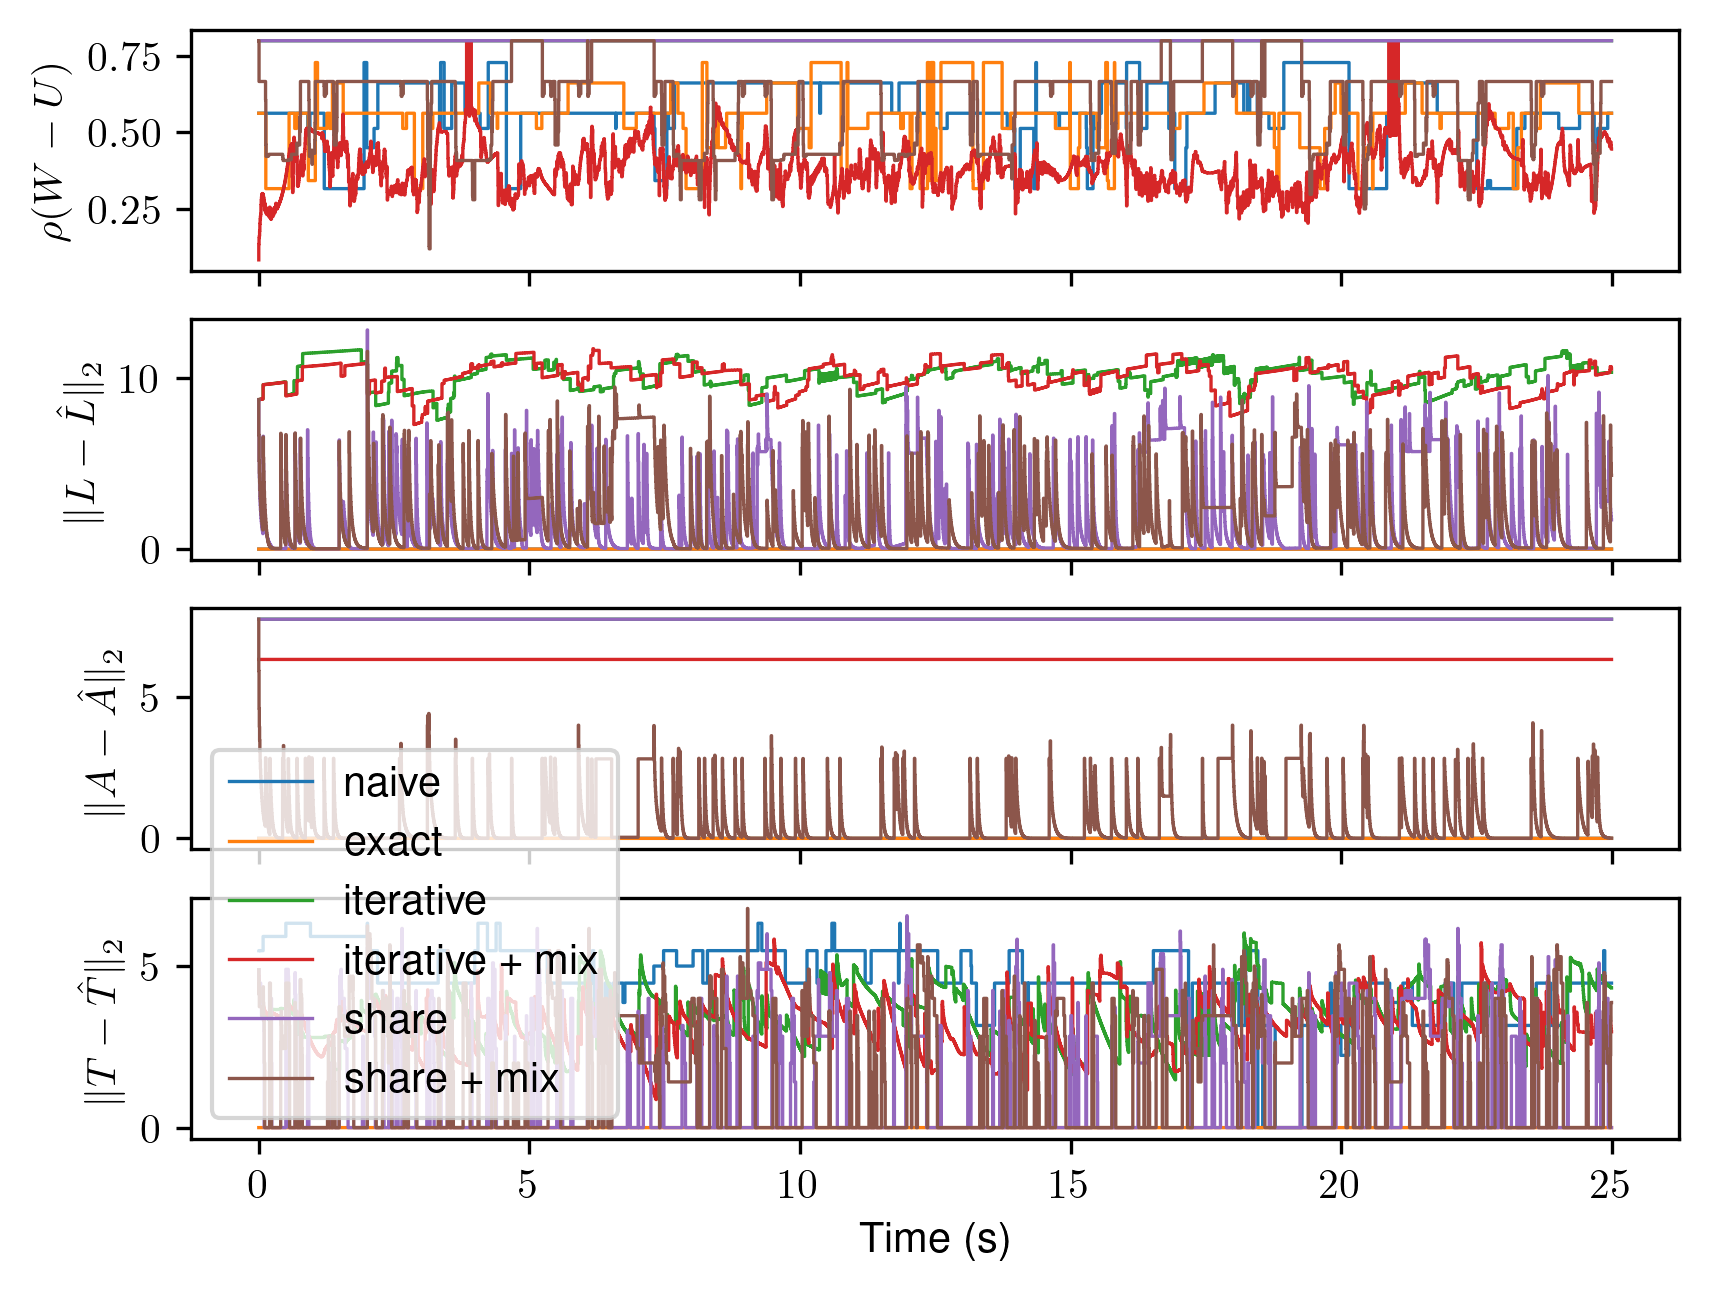
\includegraphics[width=\linewidth]{tex/small.png}
      \caption{Simulation for $B = 5$, $M = 5$, $C = 3$, $I=3$.}
      \label{fig:small}
    \end{subfigure}%
    \begin{subfigure}{0.48\linewidth}
      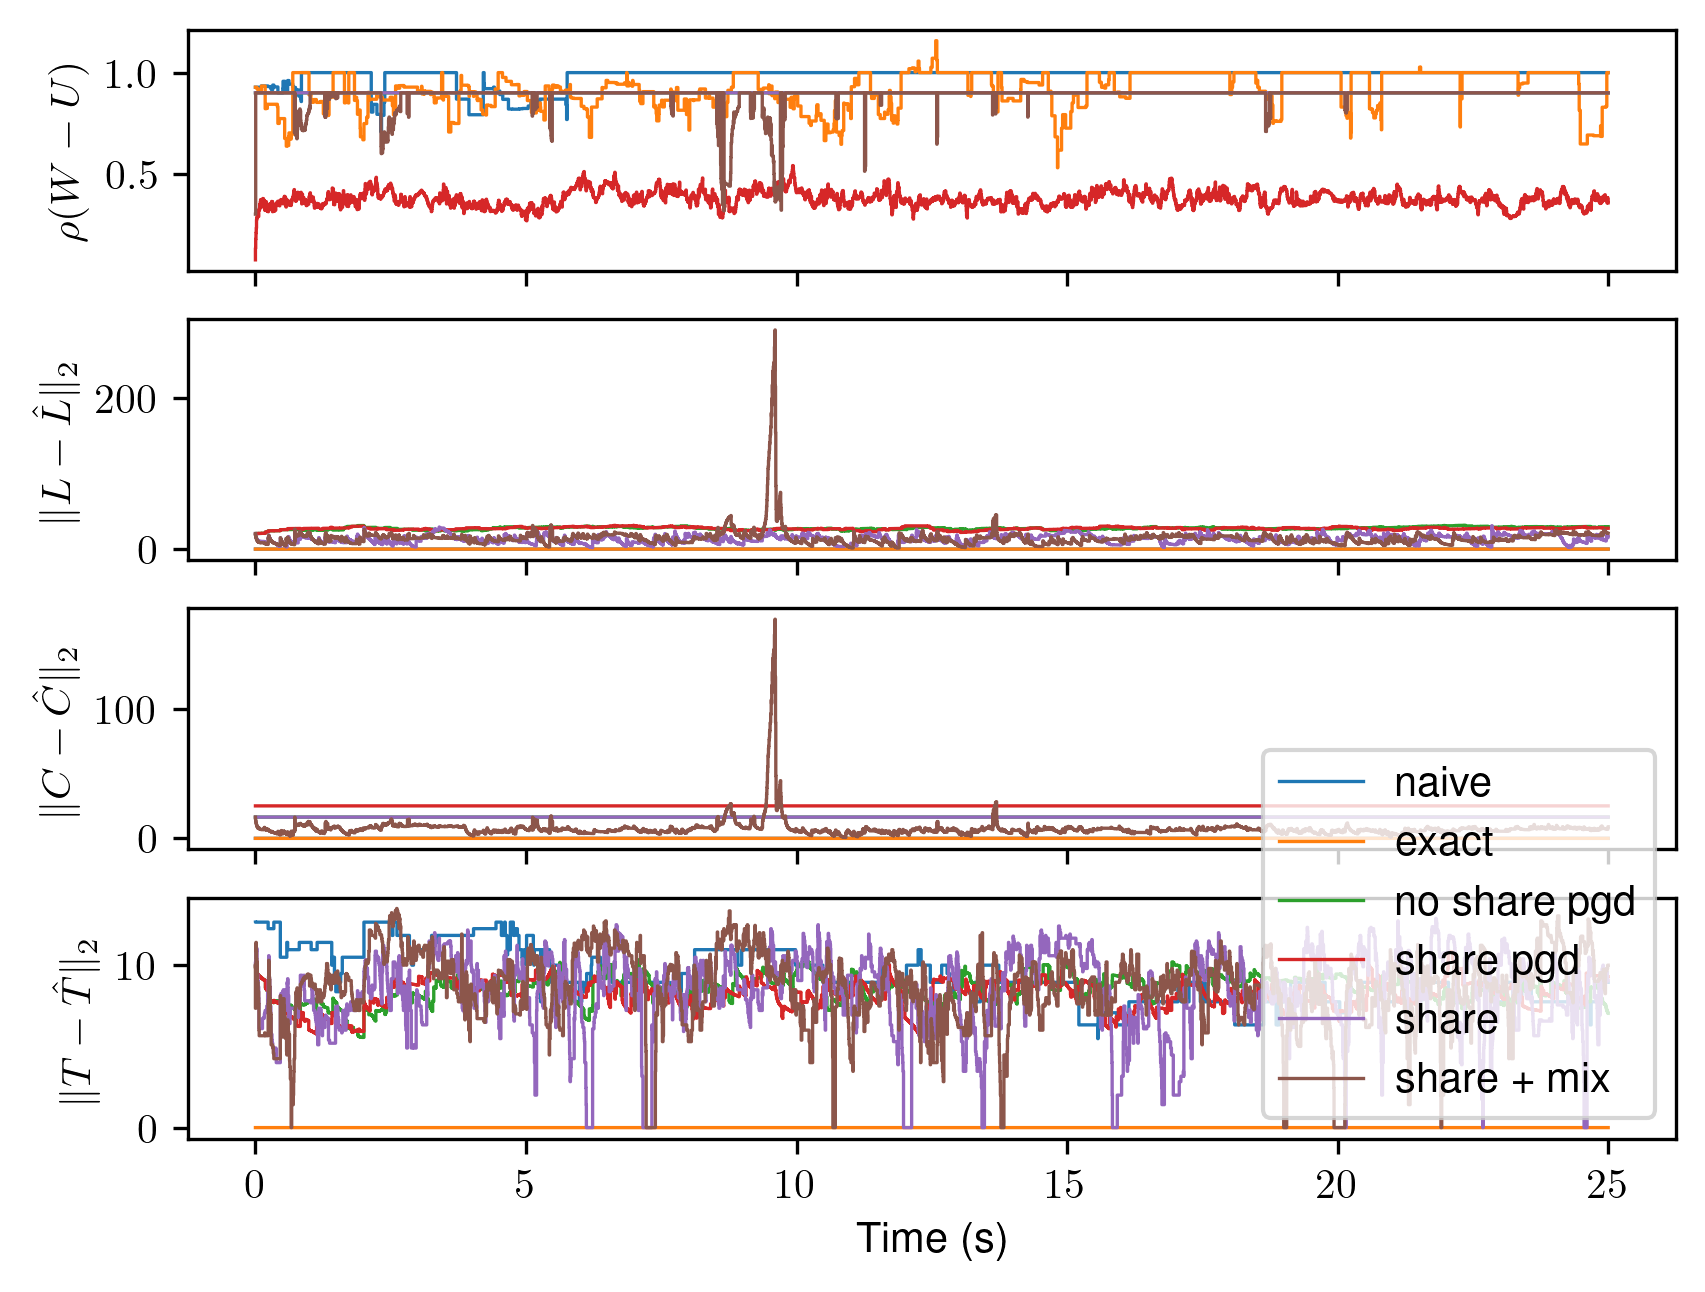
\includegraphics[width=\linewidth]{tex/big.png}
      \caption{Simulation for $B = 10$, $M = 10$, $C = 3$, $I=3$.}
      \label{fig:big}
    \end{subfigure}
    \caption{Simulation over 25 seconds for $\Delta T = 0.01$.}
    \label{fig:eff}
\end{figure}

\section*{Conclusions}
\renewcommand{\sectiontype}{Conclusions}
The objective function \eqref{eq:objective_function} which is supposed to correspond to the "exact" solution performs very well since it attains good objective values \eqref{eq:shared}, but was often outperformed by the iterative and sharing methods in our trials shown in figure \ref{fig:eff}. The performance of the iterative methods was dubious at first since the algorithm doesn't converge to an exact solution, instead arriving at a uniform task assignment matrix with a slight bias towards the preferred solution which one may round to. The iterative methods do however consistently outperform the shared methods which do arrive at exact solutions (often, given a high degree of connectivity $I$). Since the shared methods require more data to be transmitted, we find that the iterative methods always are better for this problem.
\newline

More surprising is that these methods would outperform the "exact" solution. The exact solution has demonstrated unwanted behaviour wherein two bots exchange assignments with each other back and forth until they randomly disentangle and find their own ways. This is resolved by unintended delays in the fixed point iterators which induce a hysteresis effect which prevents this problem. \newline


Co-estimation of the fastest mixing matrix on the graph greatly improves the performance of the distributed methods. The "iterative + mix" method presents a really low spectral radius, but this is since every bot locally assumes the rest of the graph to be perfectly connected. It should locally not have the fastest mixing matrix, but it doesn't seem to be a problem for performance as it enjoys a great speed-up. The shared methods also enjoy a significant speed-up. The methods appear to be very robust. \newline


\text{\bf Future work. }
The use of shifting registers in \cite{johansson2008faster} to improve the rate of convergence of linear iterators may be used to further increase the gain of the mixing matrix co-estimation. This would require one to reformulate the sharing to not use a proximal operator, which should be doable given how simple it is in form. One may of course also attempt accelerated methods. \newline


No consensus-ADMM approach was devised for this setting, and the setting was too different to offer a fair comparison to \cite{shorinwa2023distributed}. Algorithms were attempted but no great effort was expended in making it perform comparably to the presented algorithms. It would be interesting to see how fast such a method is, given that it may not be accelerated with the use of a fast mixing matrix.

\clearpage

\printbibliography

\end{document}
